\documentclass[11pt]{article}

%4pp das transps
% psnup -W415 -H273 -s.9 -b10 -d10 -c -4 05-Tecnicas_Compressao_Imagens.ps 05-Tecnicas_Compressao_Imagens.4pp.ps

\usepackage[utf8]{inputenc} % PARA USAR PALAVRAS EM PORT
\usepackage[portuguese]{babel}
\usepackage{a4wide}
\usepackage{color}
\usepackage{colordvi}
\usepackage{epsf,epsfig}
\usepackage{amsmath}
\usepackage{amsfonts}
\usepackage{enumerate}

\begin{document} 

\title{Lista de Exercícios de Sistemas de TV -- 2019-1}
\author{Luiz Felipe da S. Coelho \\ lfscoelho@ieee.org \\ DETEL -- UERJ \\ Departamento de Engenharia Eletrônica e Telecomunicações \\ Universidade do Estado do Rio de Janeiro}

\maketitle

\section{Amostragem e Subamostragem (Redução de Resolução)}

\textbf{Objetivo:} O objetivo principal das atividades desta seção é verificar empiricamente aspectos relativos à amostragem espacial de imagens e o impacto da resolução da imagem em função da distância de visualização e de captura. Temos ainda o emprego de filtros e máscaras bidimensionais. O secundário é expandir os conhecimentos sobre manipulação de matrizes e exibição de imagens usando o \textsf{Matlab}.

\subsection{Subamostragem}

\begin{enumerate}

\item \textbf{Tarefa:} Carregue a imagem \textsf{ZELDA\_S.TIF} e a mostre na tela usando 256 níveis de cinza.

\item \textbf{Tarefa:} Subamostre a imagem de 2 em cada direção (isto é, retenha somente os pixeis com índices de linha e coluna ímpares ou somente os pares) os outros pixels devem ser descartados. Obtém-se assim uma imagem com a metade das linhas e das colunas daquelas da imagem original.

\item \textbf{Tarefa:} Visualize a imagem obtida acima (apresente-a na tela). Compare a imagem obtida acima com a original.\label{sub_cor_1}

\begin{figure}[hbt!]
	\centering
	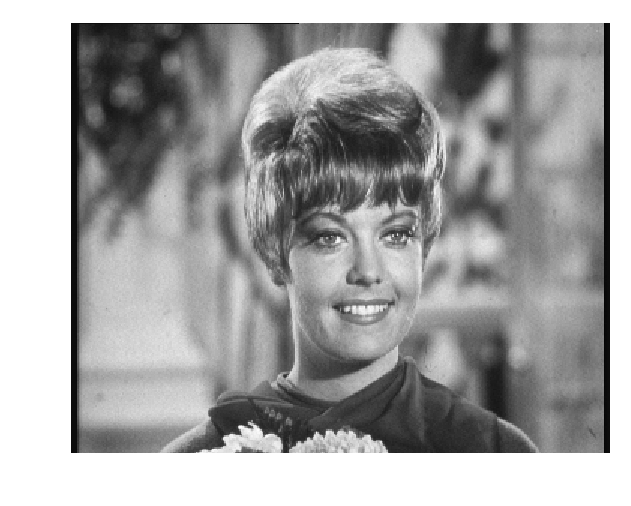
\includegraphics[scale=1]{../imgs/zelda.eps}
	\caption{Imagem \texttt{zelda$\_$s.tif}, original.}
\end{figure}

\begin{figure}[hbt!]
	\centering
	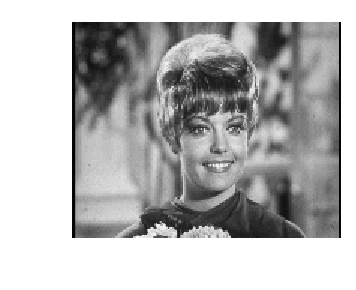
\includegraphics[scale=1]{../imgs/zelda_sub.eps}
	\caption{Imagem \texttt{zelda$\_$s.tif}, subamostrada.}
\end{figure}

\begin{itemize}
\item[\textit{Dica}:] Usar sempre o comando \textsf{truesize} para que cada pixel da imagem corresponda a um pixel na tela.

\item[\textit{Dica}:] Considere que o fator de subamostragem é $r$ para realizar as subamostragens nos itens acima. Assim retenha somente um pixel a cada $r$ pixeis nas direções horizontal e vertical.
\end{itemize}

\item \textbf{Tarefa:} \label{sub_cor_func} Faça uma função Matlab, que receba como parâmetros a imagem e $r$, e retorne a imagem subamostrada de $r$. Considere que somente a parte central da imagem será retida. Isto é, se as dimensões da imagem são $L$ e $C$ (em linhas e colunas) e se $L/r = M + resto_L$ e $C/r = N+ resto_C$, onde $L,~C$ e $r$ são inteiros, sobrarão $resto_L$ linhas e $resto_C$ colunas que deverão ser eliminadas da imagem antes de realizar a subamostragem. Essas deverão ser eliminadas retirando a quantidade de linhas e colunas necessárias no topo, fundo, esquerda e direita da imagem original. Considere a Figura \ref{fig:blocos} como ilustrativa do que deve ser feito. Observe que se $resto_L$ ou $resto_C$ forem ímpares ajustes devem ser realizados (tirando uma linha e uma coluna a mais).

\begin{figure}[h!]
\begin{center}
{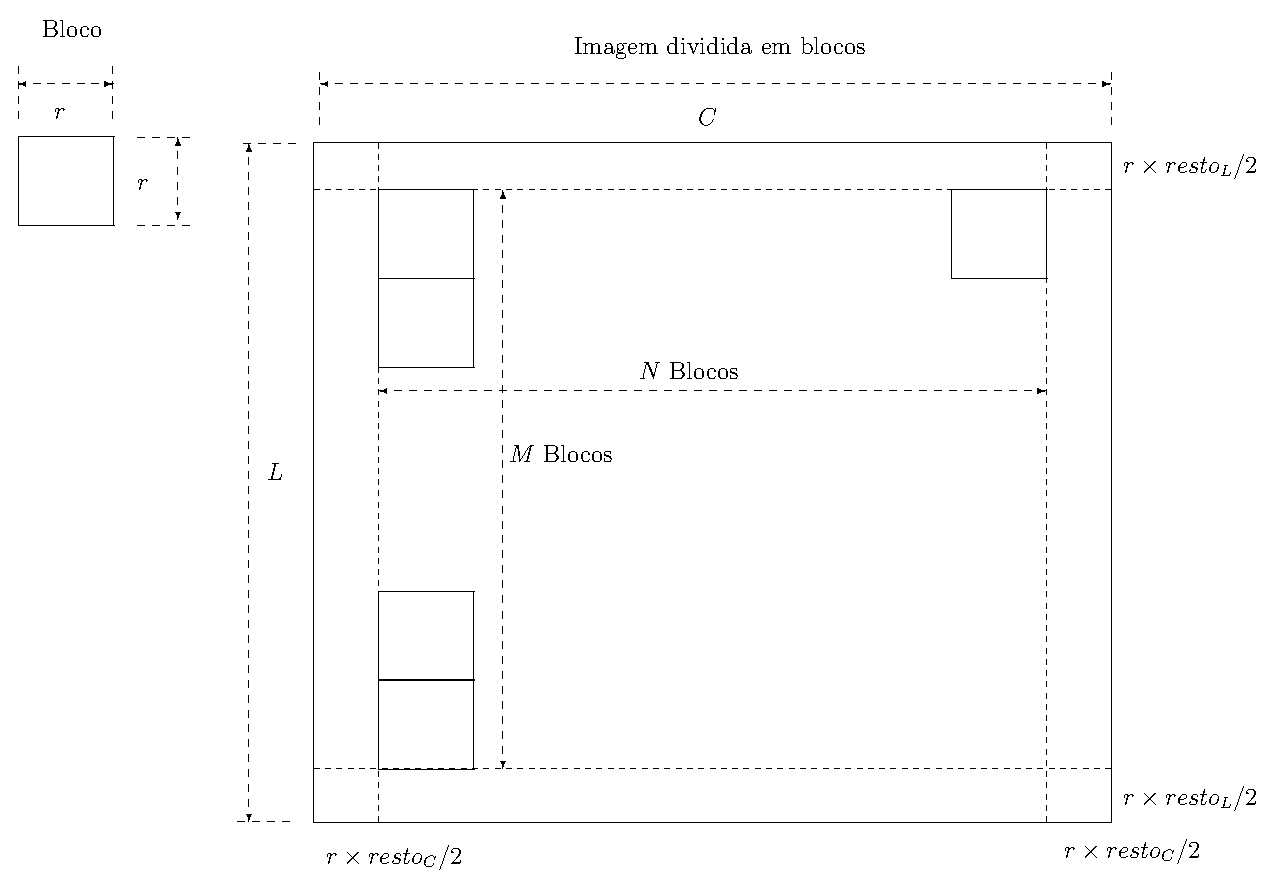
\includegraphics[width=12cm]{./blocks_div.eps}}
\caption{Divisão de uma imagem de $L\times C$ pixeis em blocos em blocos de tamanho $r\times r$.}\label{fig:blocos}
\end{center}
\end{figure}

A função que realiza a operação de subamostragem está no \textit{script} \texttt{funcs5.py}.

\item \textbf{Tarefa:} Usando a função desenvolvida acima subamostre a imagem de 4, 8, 16 e 32 em cada direção, mostrando na tela cada uma das imagens resultantes. \label{sub_cor_2}

\begin{figure}
	\centering
	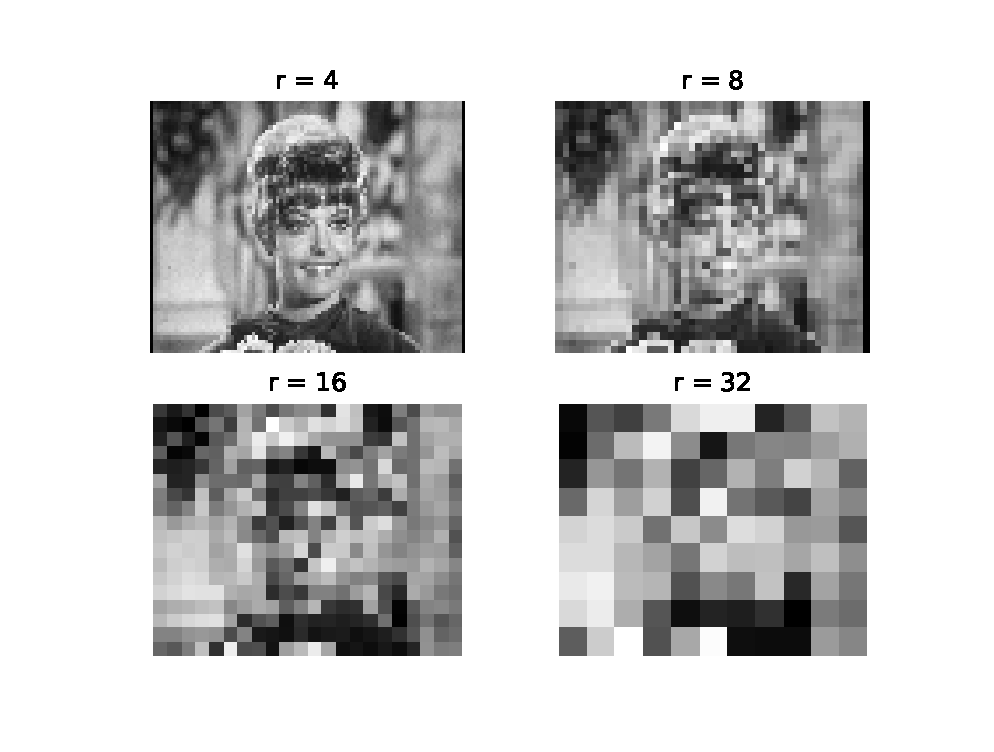
\includegraphics[scale=1]{../imgs/zelda_subs.eps}
	\caption{Quatro imagens de \texttt{zelda$\_$s.tif} subamostradas pelo fato $r = 4,~8,~16 \textrm{ e } 32$.}
	\label{fig:subs}
\end{figure}

\item \textbf{Pergunta:} Comente o que você observa. O que podemos comentar sobre o espectro de frequências de imagens subamostradas nos itens acima? Analise-o!
 \label{subcor_perg_1}
 
Pode-se observar, através da Figura \ref{fig:subs} que a qualidade visual das imagens foi drasticamente reduzida. Podemos observar também que a frequência da imagem não foi muito afetada, temos transições rápidas de pixels claros para pixels escuros.

\item \textbf{Pergunta:} Explique / averígue se as subamostragens de 4, 8, 16 e 32 solicitadas podem ser obtidas pela aplicação iterada da subamostragem de 2. Responda matematicamente. \label{subcor_perg_2}

Sim, se realizarmos o procedimento da subamostragem de 2 repetidas vezes, podemos obter os resultados das subamostragens de 4, 8, 16, 32. Isso é demonstrado no \textit{script} \texttt{pergunta7.py}

\end{enumerate}

\subsection{Subamostragem Continuação}

\begin{enumerate}

\item \textbf{Tarefa:} Repita a seção 5.1 considerando agora não a retenção de um pixel somente, mas fazendo com que os pixeis da imagem subamostrada correspondam à média dos pixeis do bloco de dimensões $r\times r$. Para isso, altere a função desenvolvida no item 5.1.\ref{sub_cor_func}. Apresente e explique essa nova função.

\begin{itemize}
\item[\textit{Dica}:] Gere uma matriz ou máscara de dimensões $r \times r$ com entradas $1$ e passe a sobre a imagem divida o resultado por $r^2$ e assim obtenha a média.

\item[\textit{Dica}:] Por exemplo, veja que a aplicação de uma máscara $A(m,n)$ de dimensões $M\times N$ (sendo $M$ e $N$ ímpares) sobre uma imagem $I(l,c)$ de dimensões $L \times C$ gera a imagem $\hat{I}(l,c)$ 
\begin{equation}
\hat{I}(l,c) = \sum_{m = \frac{-(M-1)}{2}}^{\frac{M-1}{2} } \sum_{n = \frac{-(N-1)}{2}}^{\frac{N-1}{2}} I(l+m,c+n)A(m,n),
\end{equation}
onde consideramos que a origem do eixo de coordenadas (dos índices de linhas e colunas da máscara) está no pixel central, conforme indicado na equação (\ref{eq:cite_above}).

\begin{tiny}
\begin{equation}
\hspace*{-3cm} A = \begin{bmatrix} a\left ( \frac{M\!-\!1}{2}, \frac{-\!(N\!-\!1)}{2} \right) & a\left ( \frac{M\!-\!1}{2}, \frac{-\!(N\!-\!1)}{2} \!+\!1 \right) & \!\!\cdots\!\! &  a\left ( \frac{M\!-\!1}{2},0 \right) & \!\!\cdots\!\! &  a\left ( \frac{M\!-\!1}{2}, \frac{N\!-\!1}{2} \!-\! 1 \right) & a\left ( \frac{M\!-\!1}{2}, \frac{N\!-\!1}{2} \right)  \\ 
 & &  & &  & & \\
 a\left ( \frac{M\!-\!1}{2}\!-\!1, \frac{-\!(N\!-\!1)}{2} \right) & a\left ( \frac{M\!-\!1}{2}\!-\!1, \frac{-\!(N\!-\!1)}{2} \!+\!1 \right) & \!\!\cdots\!\! &  a\left ( \frac{M\!-\!1}{2}\!-\!1,0 \right) & \!\!\cdots\!\! &  a\left ( \frac{M\!-\!1}{2}\!-\!1, \frac{N\!-\!1}{2} \!-\! 1 \right) & a\left ( \frac{M\!-\!1}{2}\!-\!1, \frac{N\!-\!1}{2} \right)  \\ 
& &  & &  & & \\
 \cdots & \vdots &  & \cdots &  &  \vdots & \cdots \\
& &  & &  & & \\
a \left (0, \frac{-\!(N\!-\!1)}{2} \right)  & \vdots &  & a(0,0) &  &  \vdots & a \left (0, \frac{N\!-\!1}{2} \right) \\ 
& &  & &  & & \\
 \cdots & \vdots &  & \cdots &  &  \vdots & \cdots \\
& &  & &  & & \\
 a\left ( \frac{-\!(M\!-\!1)}{2}\!+\!1, \frac{-\!(N\!-\!1)}{2} \right) & a\left ( \frac{-(M\!-\!1)}{2}\!+\!1, \frac{-\!(N\!-\!1)}{2} \!+\!1 \right) & \!\!\cdots\!\! &  a\left ( \frac{-\!(M\!-\!1)}{2}\!+\!1,0 \right) & \!\!\cdots\!\! &  a\left ( \frac{-\!(M\!-\!1)}{2}\!+\!1, \frac{N\!-\!1}{2} \!-\! 1 \right) & a\left ( \frac{-(M\!-\!1)}{2}\!+\!1, \frac{N\!-\!1}{2} \right)  \\ 
& &  & &  & & \\
 a\left ( \frac{-\!(M\!-\!1)}{2}, \frac{-\!(N\!-\!1)}{2} \right) & a\left ( \frac{-(M\!-\!1)}{2}, \frac{-\!(N\!-\!1)}{2} \!+\!1 \right) & \!\!\cdots\!\! &  a\left ( \frac{-\!(M\!-\!1)}{2},0 \right) & \!\!\cdots\!\! &  a\left ( \frac{-\!(M\!-\!1)}{2}, \frac{N\!-\!1}{2} \!-\! 1 \right) & a\left ( \frac{-(M\!-\!1)}{2}, \frac{N\!-\!1}{2} \right)  \\ 
\end{bmatrix} \label{eq:cite_above}
\end{equation}
\end{tiny}

\end{itemize}

A função feita está no \textit{script} \texttt{funcs5.py} e sua implementação é realizada em \texttt{52$\_$contin.py}

\begin{figure}
	\centering
	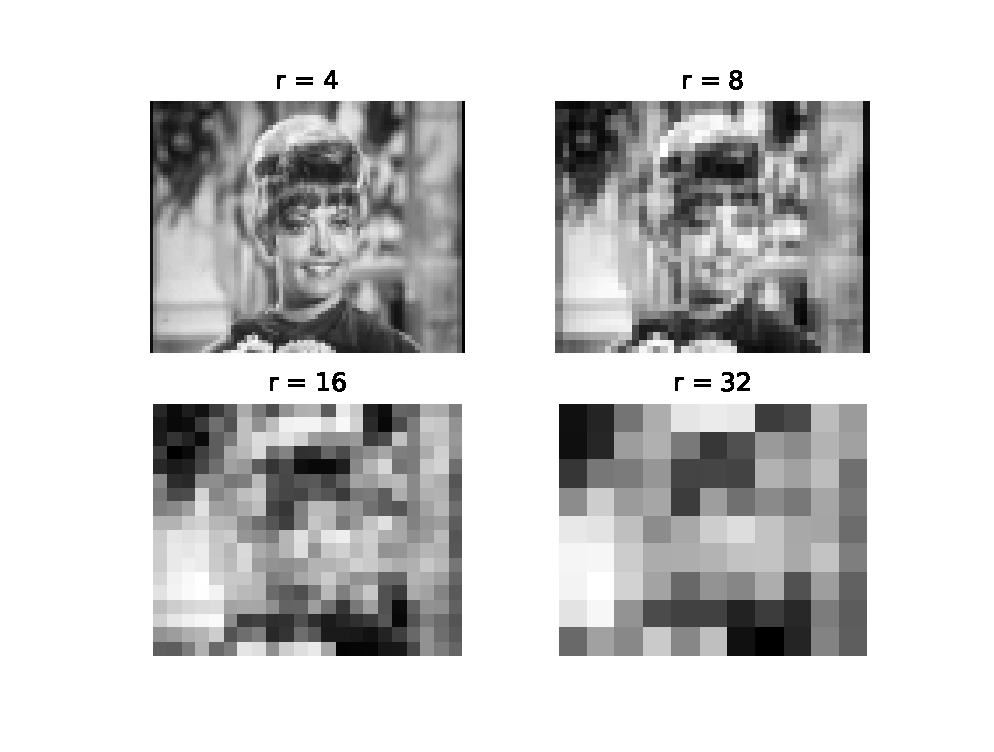
\includegraphics[scale=1]{../imgs/zelda_subsm.eps}
	\caption{Quatro imagens de \texttt{zelda$\_$s.tif} subamostradas pelo fato $r = 4,~8,~16 \textrm{ e } 32$ utilizando a média dos pixels.}
\end{figure}

\item \textbf{Pergunta:} Apresente e explique as considerações realizadas para a implementação solicitada.

Para esta realização, foi considerado que para uma imagem de dimensões $M \times N$, $M$ e $N$ são divisíveis por $r$, ou seja, na divisão dos blocos não há resto.

\item \textbf{Pergunta:} Explique / averígue se os pixeis gerados usando a forma sugerida equivalem aos que seriam gerados por uma implementação por cálculo simples da média por soma e divisão. 

\item \textbf{Pergunta:} Compare as imagens obtidas com esta nova abordagem com aquelas obtidas com a subamostragem dos itens 5.1.\ref{sub_cor_1} e 5.1.\ref{sub_cor_2} e comente as diferenças entre os procedimentos e as qualidades das imagens subamostradas observadas.

As imagens obtidas nesse procedimento têm transições mais suaves, o que as tornam um pouco mais nítidas que aquelas dos processos anteriores.

\begin{itemize}
\item[\textit{Dica}:] A passagem de uma máscara sobre uma imagem pode ser obtida a partir da convolução. O \textsf{Matlab} fornece a função \textsf{conv2} para a convolução bidimensional. 

Sejam $F(m,n)$ e $G(m,n)$ duas sequencias bidimensionais, isto é, $m$ e $n$ $\in \mathbb{Z}$, a convolução 2D dessas sequencias é
\begin{footnotesize}
\begin{equation}
F(m,n)*G(m,n) = G(m,n)*F(m,n) = \sum_k\sum_l F(k,l)G(m-k,n-l) = \sum_l\sum_k G(k,l)G(m-k,n-l).
\end{equation}\end{footnotesize}
Observe que a imagem resultante da convolução de uma imagem de dimensões $M\times N$ por um filtro de dimensões $r\times r$ tem dimensões $(r+M-1) \times (r+N-1)$. 
\end{itemize}

\item \textbf{Pergunta}: Sendo assim, explique como a aplicação de uma máscara a uma imagem pode ser obtida a partir da convolução bidimensional. 

\begin{itemize}
\item[\textit{Dica}:] Não se esqueça de considerar dois aspectos:

\begin{itemize}
\item[a)] Quais transformações deverá sofrer uma máscara de forma a gerar uma matriz $A$ que pode ser convoluída bidimensionalmente com a imagem e obter o mesmo resultado da aplicação da máscara?

\item[b)] Qual a eliminação de linhas e colunas a ser aplicada à imagem resultante da convolução de forma a obter uma imagem que possua as mesmas dimensões da imagem original, de forma tal que a área da imagem resultante seja o mais próxima possível da área da imagem original?
\end{itemize}
\end{itemize}

\end{enumerate}
\end{document}